\documentclass[11pt,a4paper,twoside]{article}
\usepackage{tascar}
\pagenumbering{arabic}
\pagestyle{empty}
\showtutorialtrue
\begin{document}
\setcounter{tutorial}{5}
\begin{tutorial}{Interactive motion-tracked binaural rendering}{Seminar room}
  Create an interactive ``multi-player'' radio drama.
  Walk and talk through your virtual environment.  
  You will use multiple independent receivers, motion controlled by
  game controllers and wireless head tracking.

\begin{learnitems}
\item How to apply head motion tracking to virtual binaural receivers
\item Delay compensation for own-voice processing
\item How to connect {\em everything} (says Maartje)
\end{learnitems}

\begin{appitems}
\item Interactive auralization
\item In-ear monitoring
\end{appitems}

~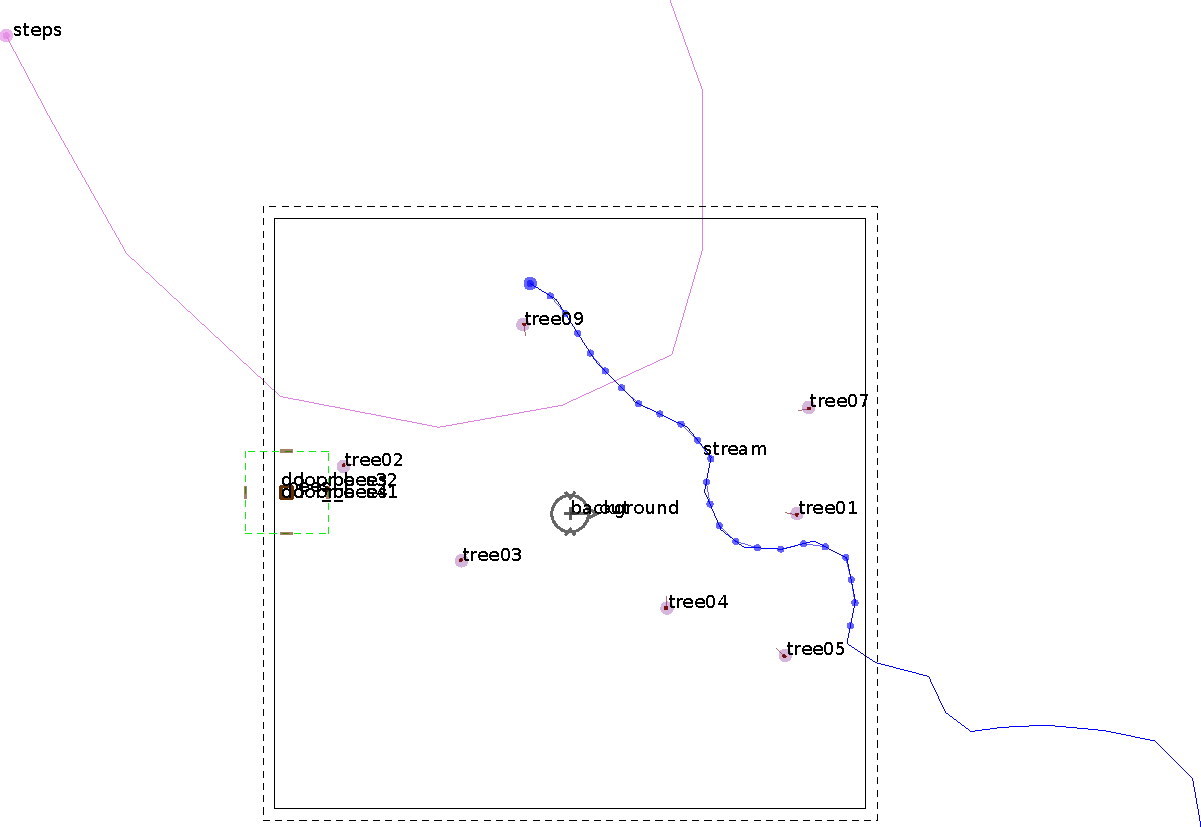
\includegraphics[width=0.6\columnwidth]{t6_map.pdf}\hfill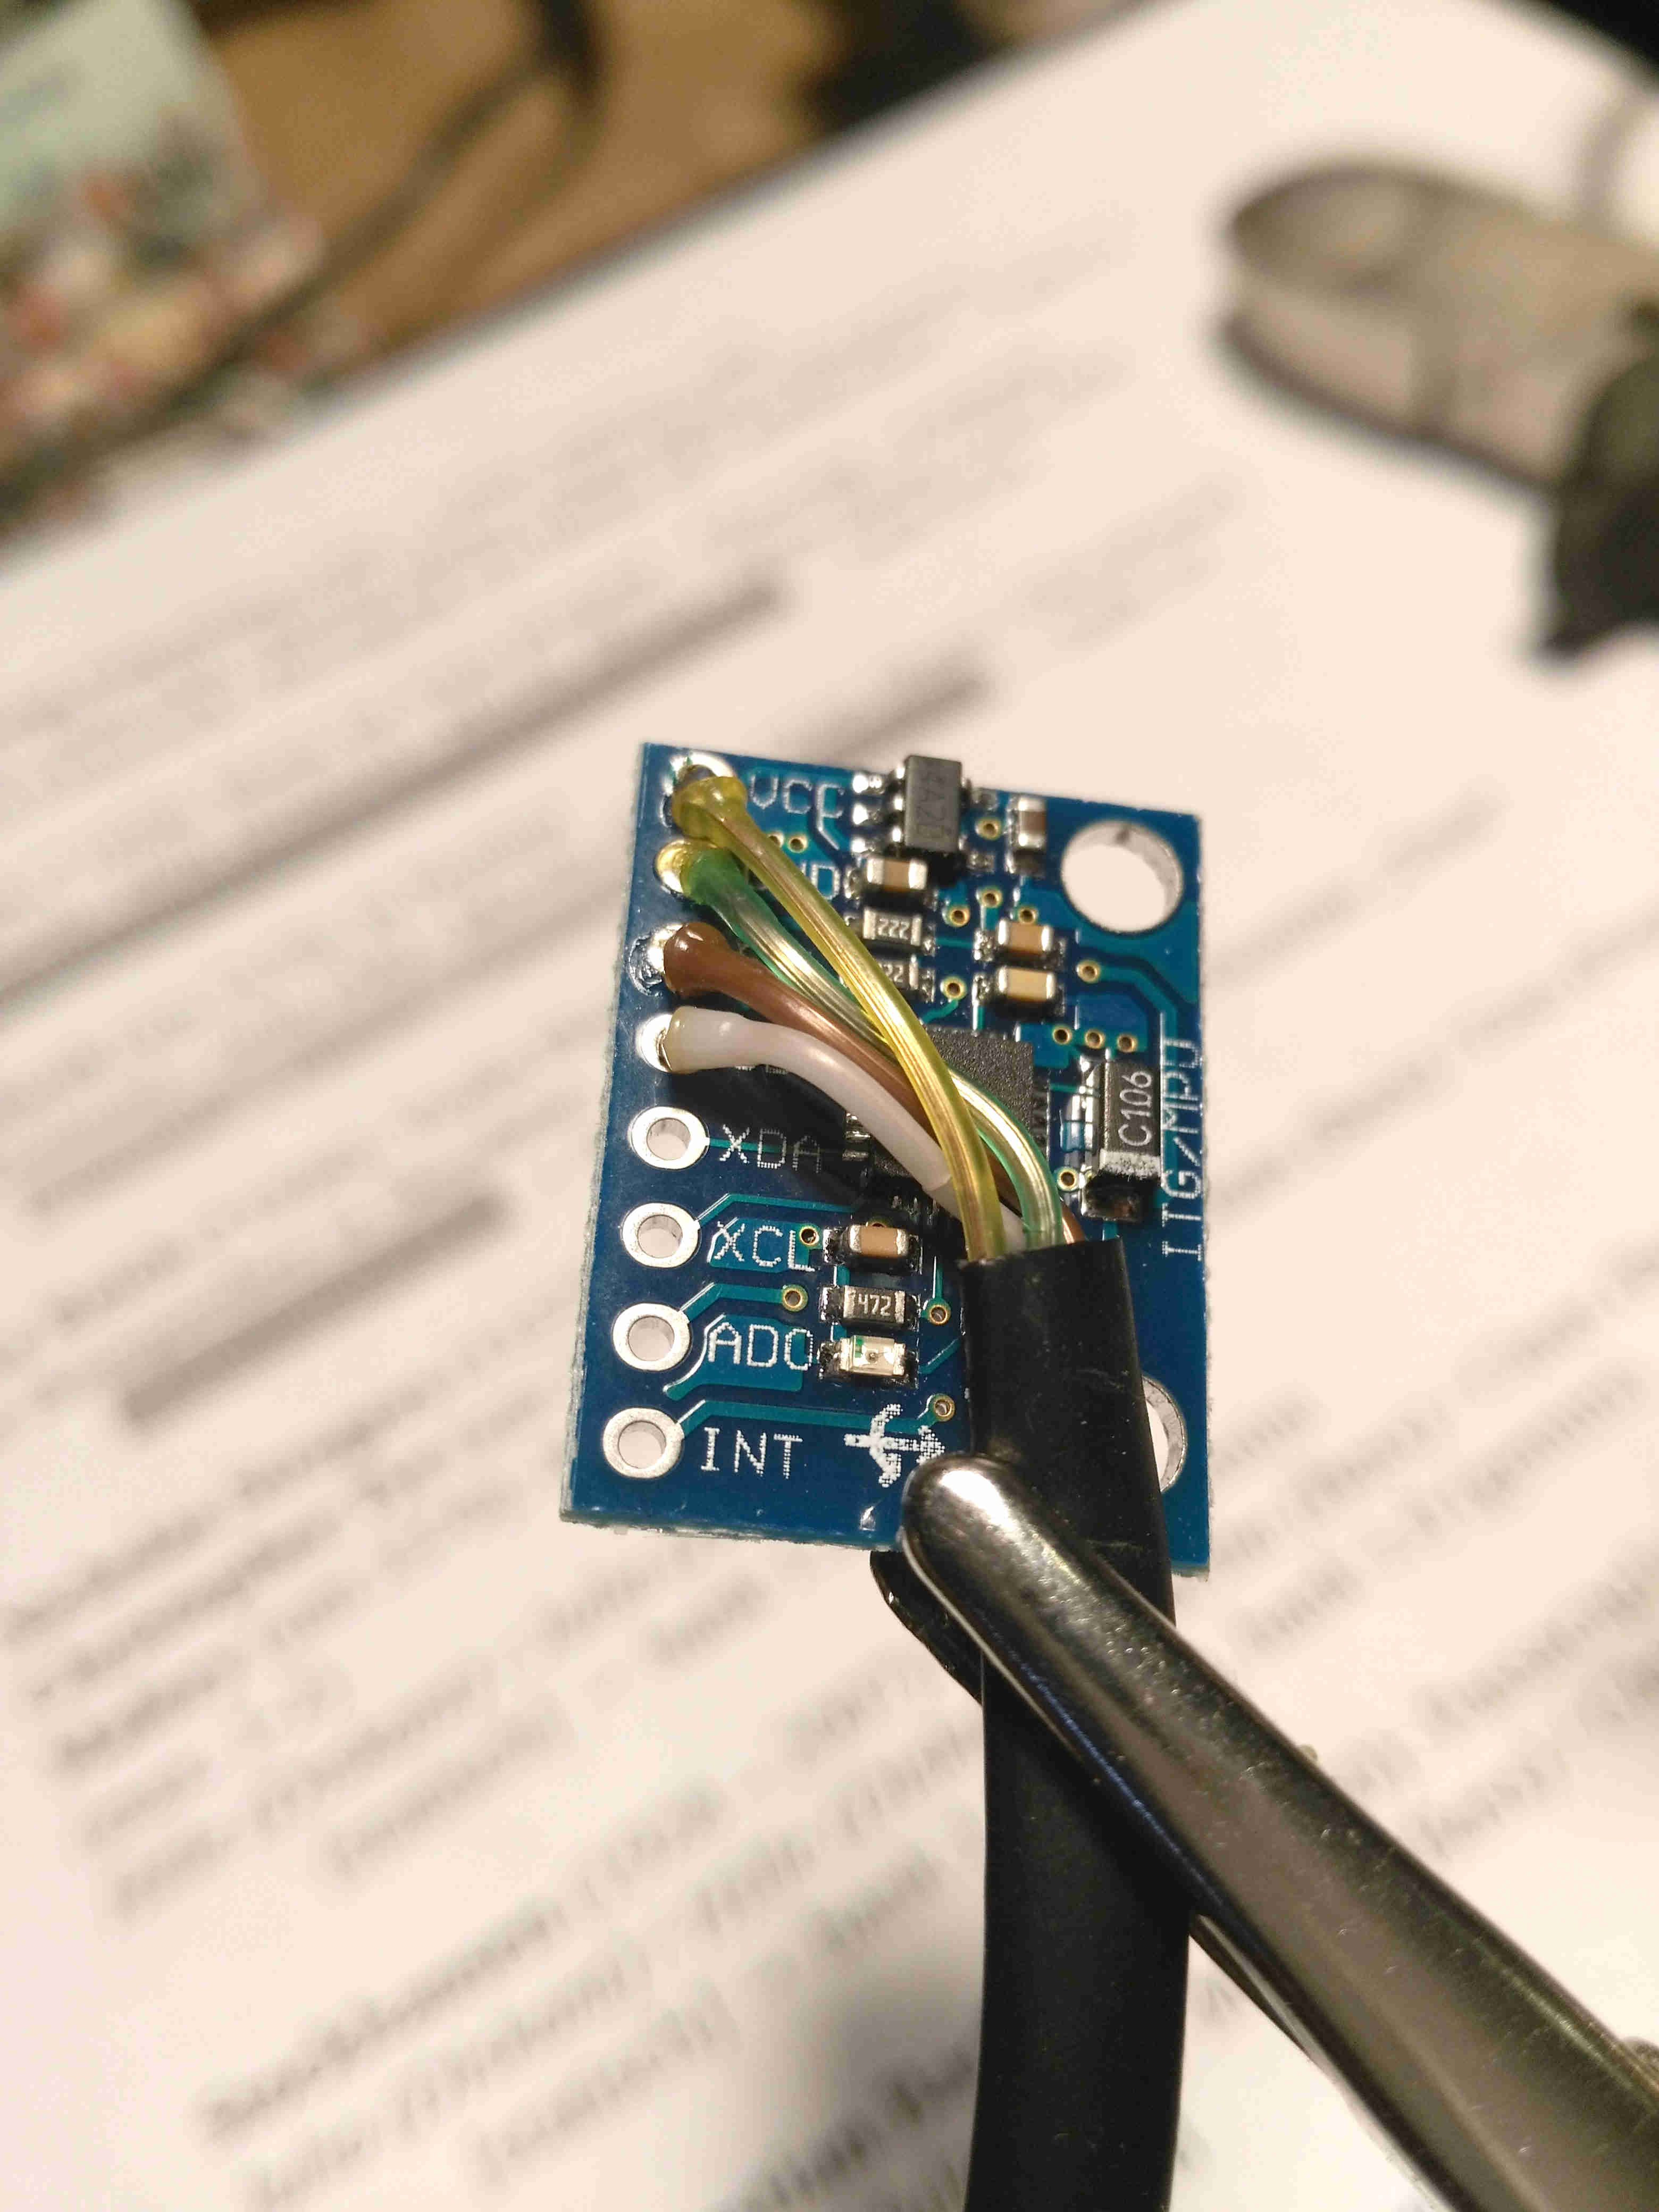
\includegraphics[width=0.35\columnwidth,trim=0 0 0 1800px]{mpu6050.jpg}~

\end{tutorial}
\end{document}
